\documentclass[10pt]{article}         %% What type of document you're writing.

%%%%% Preamble

%% Packages to use

\usepackage{amsmath,amsfonts,amssymb,mathtools}   %% AMS mathematics macros
\usepackage{graphicx}
\usepackage{caption}
\usepackage{subcaption}
\usepackage{tikz}
\usetikzlibrary{decorations.pathreplacing,matrix}
\usetikzlibrary{decorations.pathmorphing}
\usetikzlibrary{decorations.text}

\tikzset{ 
  table/.style={
    matrix of math nodes,
    row sep=-\pgflinewidth,
    column sep=-\pgflinewidth,
    nodes={rectangle,text width=3em,align=center},
    text depth=1.0ex,
    text height=1.0ex,
    nodes in empty cells,
    left delimiter=[,
    right delimiter={]},
  }
}

\DeclarePairedDelimiter\abs{\lvert}{\rvert}%
\DeclarePairedDelimiter\norm{\lVert}{\rVert}%
\newtheorem{exmp}{Example}[section]
%% Title Information.

\title{A better visual odometry with bundle adjustment and uncertainty modeling}
\author{Ilan Shimshoni, Ehud Rivlin, Alex Kreimer}

\begin{document}

\maketitle

\abstract{This draft summarizes the work I did so far: implemented
  bundle adjustment which allows to take uncertainties into account
  while estimating motion parameters and also implemented a simulated
  environment which allows to easily inject various types of noise and
  verify the behaviour of the algorithms.}

\section{Notation}

This section makes definitions that are used throughout the document.

Let the camera $j$ be parameterized by a vector $a_j$, $j=1,\dotsc,n$,
and 3d the point $i$ by vector $b_i$, $i=1,\dotsc,m$.  We assume
calibrated cameras and thus parations that are used throughout the document.

Let the camera $j$ be parameterize only the extrinsic camera
parameters.  The rotation is represented by three Euler angles and the
translation is taken ``as is''. \emph{Parameter} vector
$\theta\in R^M$ is defined as:
$\theta=[a_1^T,\dotsc,a_n^T,b_1^T, \dotsc,b_m^T]^T$.

$x_{ij}\in\mathcal{R}^k$ denotes the image coordinates 3d point $i$ as
seen in image $j$.

\emph{Measurement} vector is defined by image observations:
$X = [x_{11}^T,\dotsc, x_{1m}^T,\allowbreak
x_{21}^T,\dotsc,x_{2m}^T,\dotsc,x_{n1}^T,\dotsc,x_{nm}^T]$,
$X\in\mathcal{R}^N$ and it is accompanied by its covariance data
$\Sigma_X=diag(\Sigma_{x_{11}},\dotsc,\Sigma_{x_{nm}})$,
$\Sigma_{ij}\in \mathcal{R}^{k\times k}$. In case of missing
measurement it just disappears from the measurement vector, so the
indices may have ``holes'' in them.

\emph{Prediction} vector is a function of the parameter vector $\theta$:
$\hat{X} = [\hat{x}_{11}^T,\dotsc,\hat{x}_{1m}^T,\allowbreak
\hat{x}_{21}^T,\dotsc,\allowbreak
\hat{x}_{2m}^T,\dotsc,\hat{x}_{n1}^T,\dotsc,\hat{x}_{nm}^T]$,
s.t. $\hat{x}_{ij} =f_{ij}(P)$.

Bundle adjustment is problem of finding a set of parameters that make
observations in different views as ``consistent'' as possible.
Different formulations of consistency are possible with maximul
likelihood one dominating the literature.

\section{Problem Formulations}

\subsection{Maximum Likelihood}

Maximum likelihood estimator seeks to maximize the likelihood of the
data given the parameters:
\[
\theta_{ML} = \underset{\theta}{\text{argmax}}\ p(X|\theta)
\]
We assume that the measurements adhere to the following statistical
model:
\[
x_{ij} = \hat{x}_{ij}+\epsilon_{ij}
\]
where $\hat{x}_{ij}$ is the model prediction, $\epsilon_{ij}$ is a
Gaussian noise with zero mean and a known covariance
$\Sigma_{ij}$. Thus $x_{ij}$ is a $k$-vector Gaussian random variable
with mean $\hat{x}_{ij}$ and covariance matrix $\Sigma_{ij}$. Hence
the probability density of $x_{ij}$ given $\theta$ is:
\[
p(x_{ij}|\theta)=\frac{1}{\sqrt{(2\pi)^n\left|\Sigma_{ij}\right|}}\exp^{-(x_{ij}-\hat{x}_{ij},\Sigma_{ij}^{-1}(x_{ij}-\hat{x}_{ij}))/2}
\]

Thus ML estimator is:
\begin{equation}\label{eq:ml}
\theta_{ML} = \underset{\theta}{\text{argmax}}\ p(X|\theta) =
\underset{\theta}{\text{argmax}} \prod_{i,j} p(x_{ij}|\theta)
=\underset{\theta}{\text{argmin}}\ \sum_{ij}\left\| x_{ij}-\hat{x}_{ij}\right\|_{\Sigma_{ij}}
\end{equation}

This is typical formulation of BA procedure found in the
literature. It accounts for the uncertainty in the measurements while
the prior distribution of the parameters is assumed to be uniform.

\emph{Note}: if the covariances are all of the form $\Sigma_{ij}=a I$
then
\[
\underset{\theta}{\text{argmin}}\ \sum_{ij}\left\|
  x_{ij}-\hat{x}_{ij}\right\|_{\Sigma_{ij}} = \underset{\theta}{\text{argmin}}\ \sum_{ij}\left\|
  x_{ij}-\hat{x}_{ij}\right\|_2^2
\]
thus minimization of unweighted reprojection errors implicitly assumes
equal measurement covariance.

\subsection{Maximum a posteriori probability}

Now we assume a joint distribution $p(X,\theta)$ and seek to maximize
the posterior distribution on the parameters
\[
\theta_{MAP} = \underset{\theta}{\text{argmax}}\ p(\theta|X)= \underset{\theta}{\text{argmax}}\ p(X|\theta)p(\theta)
\]

In case of a Gaussian zero mean and a known covariance  prior over the parameters
\[
\theta_{MAP} = \underset{\theta}{\text{argmin}}\ \sum_{ij}\left\|
  x_{ij}-\hat{x}_{ij}\right\|_{\Sigma_{ij}} + \sum_i
\left\|b_i-b_i^0\right\|_{\Sigma_{b_i}} + \sum_j\left\|a_j-a_j^0\right\|_{\Sigma_{a_j}}
\]
\emph{Note} Motion priors may be modelled as a distribution over
the camera extrinsic parameters while structure uncertainty may be
modeled as a prior distribution over the structure parameters.

\subsection{A choice of parameterization}

3d points are represented by 3 vectors $b_j = X_j = [X_j,Y_j,Z_j]^T$.
Camera motion is parameterized by a 6 vector
$a_i = [r_x,r_y,r_z,t_x,t_y,t_z]$.  Rotations are parameterized using
Euler angles $ R = R_z(r_z)R_y(r_y)R_x(r_x)$.  Translation is
represented by a 3 vector $ dt = [d_x,d_y,d_z]^T$. Left (right) camera
$i$ projection of 3d point $X_j$:
$$
\begin{aligned}
  \hat{x}^{(l)}_{ij} &= \pi^{(l)}(a_i,b_j) = K[R^{(l)}(a_i)\ T^{(l)}(a_i)]b_j\\
  \hat{x}^{(r)}_{ij} &= \pi^{(r)}(a_i,b_j) = K[R^{(r)}(a_i)\
  T^{(r)}(a_i)]b_j
\end{aligned}
$$

\section{Implementation}

\begin{figure}
  \centering
  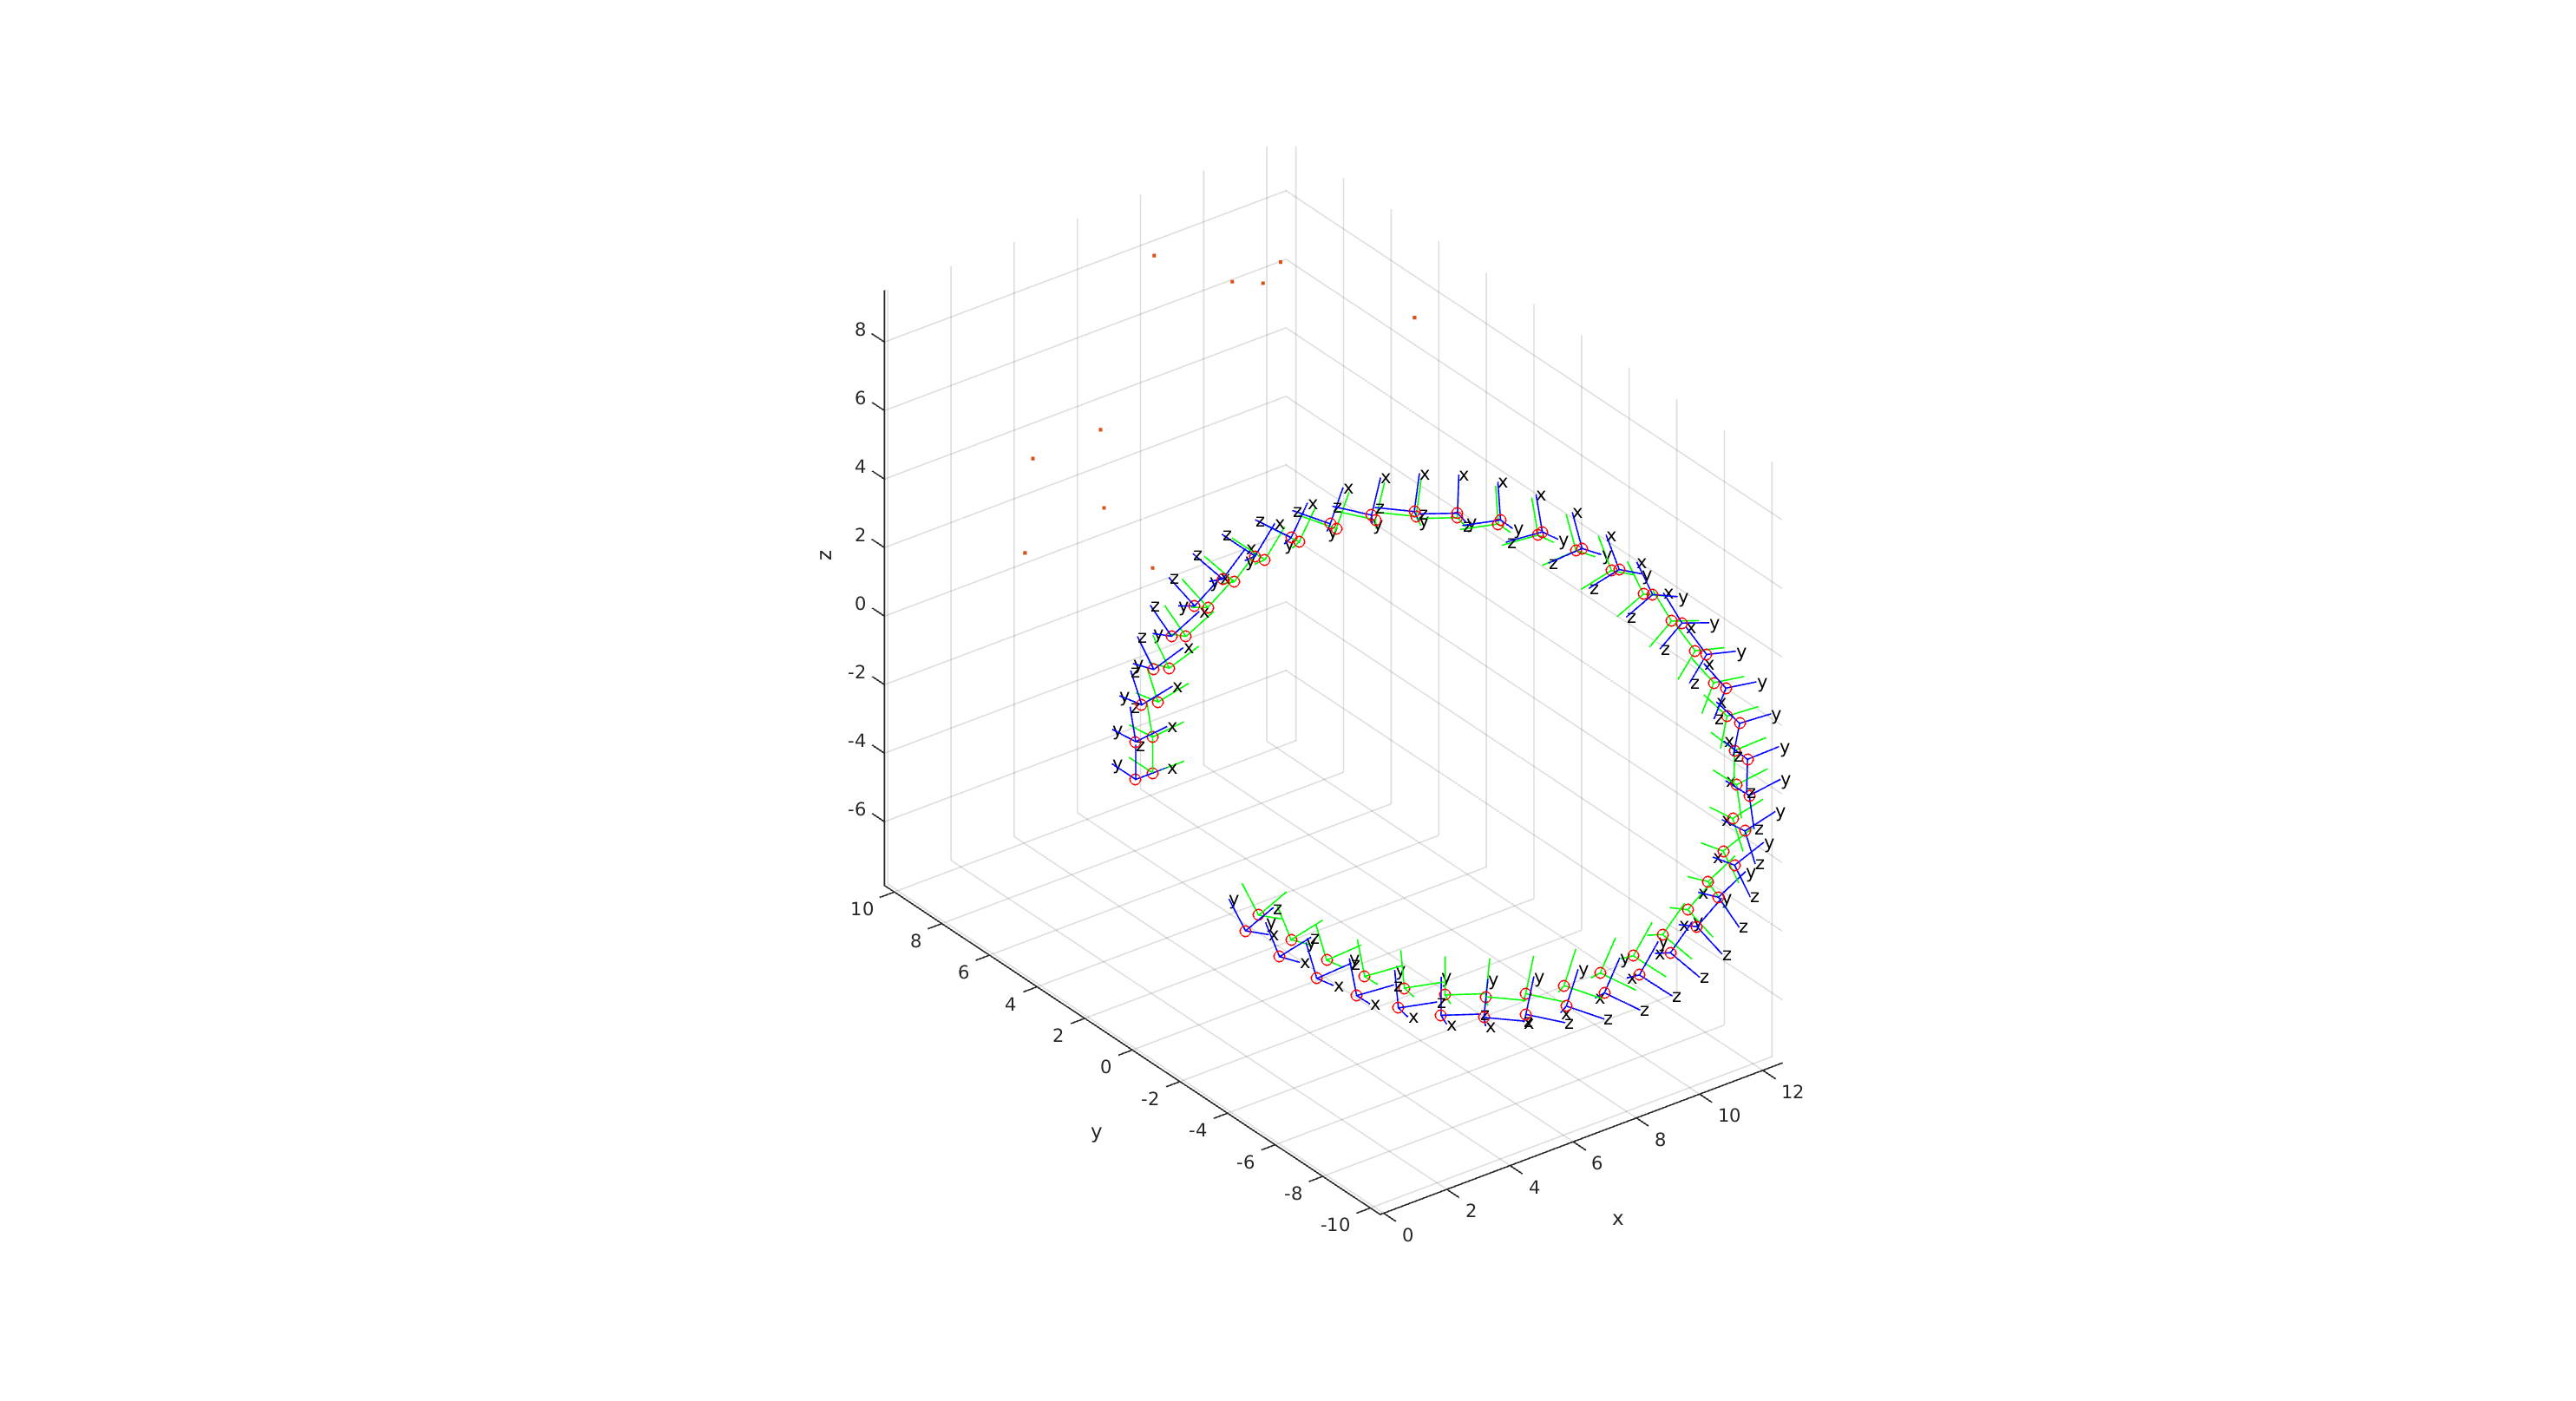
\includegraphics[width=1.5\textwidth]{camera_poses}
  \caption{A possible simulation scene that depicts stereo camera
    motion and scene structure.}
  \label{fig:poses}
\end{figure}%
\begin{figure}
  \centering
  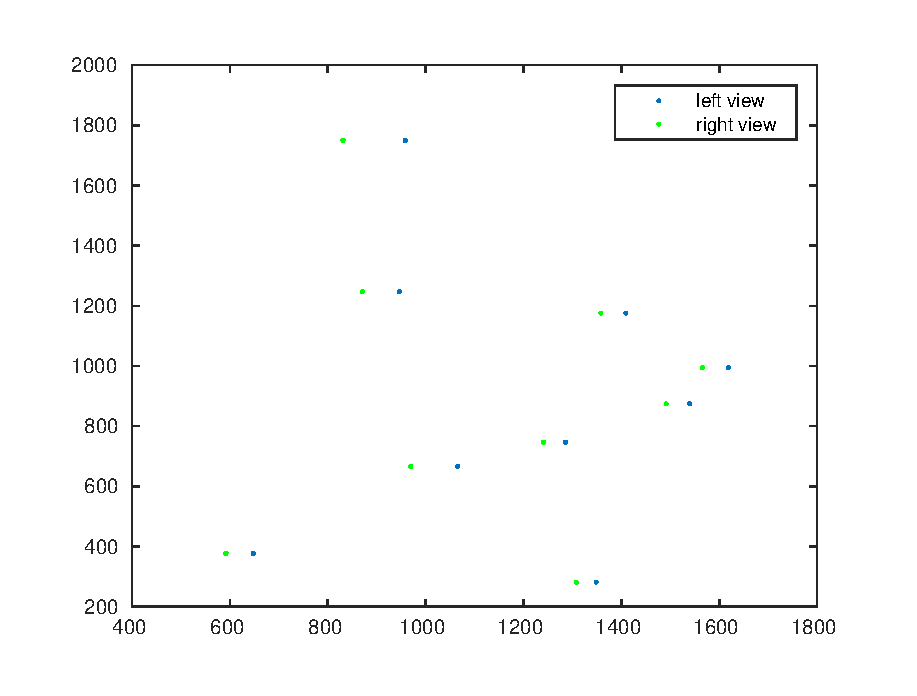
\includegraphics[width=0.9\textwidth]{camera_proj}
  \caption{Scene projection as seen by one of the stereo pairs}
  \label{fig:proj}
\end{figure}

We implemented a simulator that allows to move the camera in a
predefined (known) way.  As they move the cameras observe a set of known 3d
points. Parameter estimation procedure is used to estimate the motion
and/or structure which may be compared to the true parameter value.

Figure ~\ref{fig:poses} depicts a possible scene with cameras
and structure. Figure ~\ref{fig:proj} shows a typical image seen by a
stereo rig in the simulator.

Camera motion and structure parameters are estimated in 3 steps. Note
that this procedure is not intended to be optimal but rather to get a
feeling of what various parameter estimation schemes are capable of on
the synthetic data:
\begin{itemize}
\item Camera motion between each subsequent stereo frames is
  estimated. We triangulate both sets of observations to obtain the 3d
  in both frames.  Then we solve $R=\underset{\Omega}{\text{argmin}}\
  \norm{A\Omega - B}_F\ \text{s.t.}\ \Omega^T\Omega=I$. If $M=A^TB$
  and $M=U\Sigma V^*$ is its SVD decomposition, then $R=UV^*$
\item Single step re-projection minimization $\theta =
  \underset{\theta}{\text{argmin}}\ \norm{X-\hat{X}(\theta)}^2_2$.
  The optimization is solved using LM algorithm, the result of the
  previous section is used as an initial guess
\item We refine the parameters from previous step, by solving problem
  ~\ref{eq:ml} (e.g., bundle adjustment over all frames and
  structure).  The parameters that are obtained as an output of this
  step are our best estimate. Bundle adjustment is performed twice,
  once with all unit co-variances another time with real co-variance
  information.
\end{itemize}

\begin{figure}
  \centering
  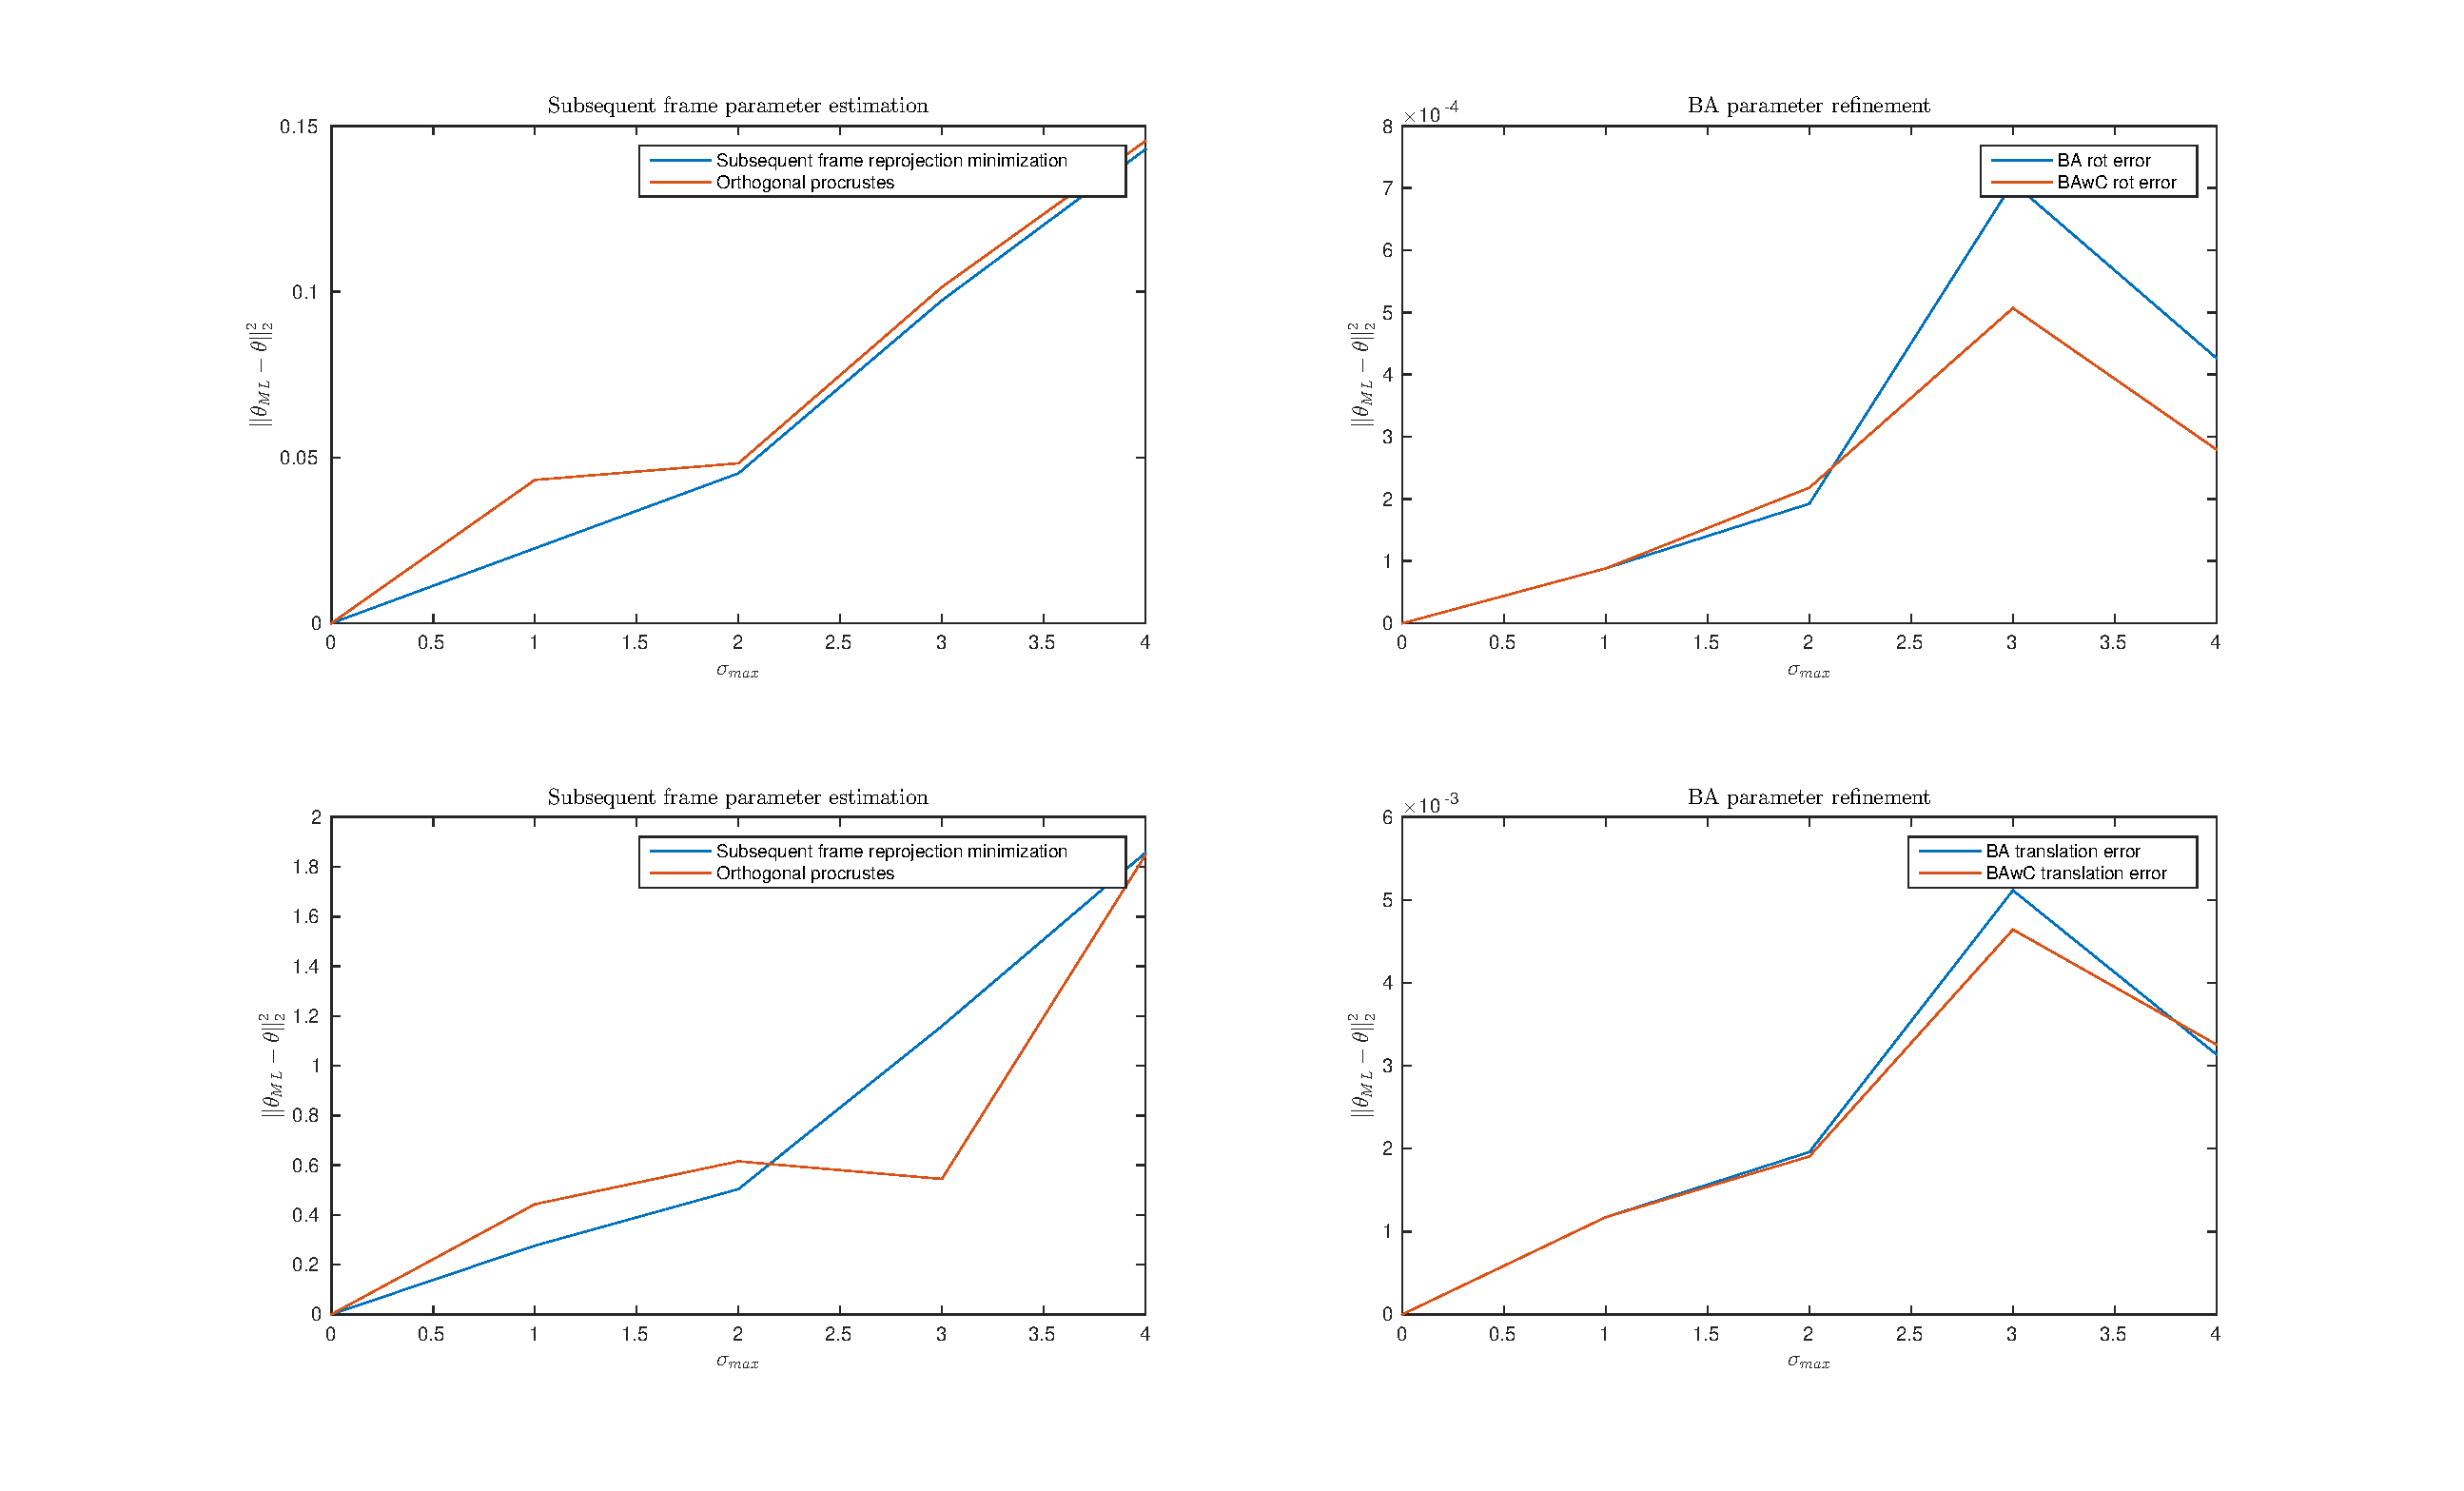
\includegraphics[width=1\textwidth]{graphs}
  \caption{First column presents results for subsequent frame motion
    estimation, while second column shows results for BA performed
    over all frames seen up to this point.  The results are averaged
    over 10 camera motions.  Each camera observed 20 3d points.  No
    outliers were introduced into the experiment. BAwC stands for
    bundle adjustment with co-variance, while BA stands for bundle
    adjustment with all unit co-variances}
  \label{fig:graphs}
\end{figure}

We perform the above parameter estimation procedure a number of times
each time adding a noise to the pixel measurements. For each
experiment we set a maximum value for standard deviation of noise,
$\sigma_{max}\in \{1\dotsc 4\}$. For each coordinate of each
measurement we generate $\sigma \sim U[0,\sigma_{max}]$ and then
perturb the measurement coordinate by $\epsilon \sim N(0,\sigma^2)$.

Figure ~\ref{fig:graphs} presents results.

\section{Essential bundle adjustment}

\subsection{Estimation of motion parameters}
$R$ describes world frame in terms of camera frame. $q_1$ is a
direction from $C_2$ to $C_1$ described in $C_2$.

Thus for every pair of correspondences $x,x'$; $(C_1,C_2)$ holds
\[
x'^TK^{-1}[q]_{\times}RK^{-1}x=0
\]

We define the following objective (includes multiple features):
\[
F(q,R) = \sum_i^N{ [x_i'^TK^{-1}[q]_{\times}RK^{-1}x_i]^2 } + [\lambda(q^Tq-1)]^2
\]

\begin{tikzpicture}
\draw [help lines, dotted] (0,0) grid (4,3);
\draw [dashed] (0,0) -- (2,2);
\draw [->] (2,2) -- (1.5,1.5);
\node [left] at (1.5,1.5) {$R,q_1$};
\draw [red, fill] (0,0) circle [radius=0.05];
\node [below left] at (0,0) {$C_1$};
\node [above left] at (2,2) {$C_2$};
\draw [red, fill] (2,2) circle [radius=0.05];
\end{tikzpicture}

\subsection{Gauss Newton iteration}

Let $r(q(t_x,t_y,t_z),R(r_x,r_y,r_z)) \in \mathbf{R}^{N+1}$ be defined as (we further omit the parameterization of the translation and the rotation):

\begin{align*}
  r_i &= x_i'^TK^{-1}[q]_{\times}RK^{-1}x_i\\
  r_{N+1} &= \lambda(q^Tq-1)
\end{align*}

So,
\begin{align*}
F(q,R) &= r^Tr = \sum_i^{N+1} r_i^2\\
(\nabla F)_j& = \sum_i^{N+1} 2 r_i (\nabla r_i)_j\ \text{and thus, } \nabla F = 2J^Tr\quad\text{where, } J=[\nabla r_1 \nabla r_2 \ldots \nabla r_{N+1}]^T\\
(\nabla^2 F)_{jk} &= 2\sum_i^{N+1} (\nabla r_i)_k (\nabla r_i)_j+r_i(\nabla^2 r_i)_{jk}\ \approx 2\sum_i^{N+1} (\nabla r_i)_k (\nabla r_i)_j\\
\nabla^2 F &\approx 2J^TJ
\end{align*}

\subsection{Dogleg algorithm}
The algorithm sets a trust region radius $\Delta$.  Possible search
direction is $p = p_{sd}+\lambda(p_N-p_{sd})$ where $\lambda \in [0,1]$ (a compromise
between steepest descent and Newton directions):
\[
\lambda^*=\underset{\lambda}{\text{argmax}}\ \norm{p}\ \text{s.t.}\ \norm{p}\leq\Delta
\]

\begin{align*}
  \norm{p}^2 &= \norm{p_{sd}+\lambda(p_N-p_{sd})}^2\\
  &= \norm{p_{sd}}^2 +2\lambda p_{sd}^T(p_N-p_{sd})+\lambda^2\norm{p_N-p_{sd}}^2 = \Delta^2
\end{align*}

This is a quadratic equation in $\lambda$ and $\lambda^* =
\frac{-b+-\sqrt{b^2-4ac}}{2a}$, $a=\norm{p_N-p_{sd}}^2$, $b=2p_{sd}^T(p_N-p_{sd})$, $c= \norm{p_{sd}}^2-\Delta^2$


\subsection{Stereo}
Let $C_i$ and $C_i'$ be the locations of the left/right camera at time
$i$. The rig is moving rigidly and we are interested to recover this
motion.

Epipolar constraint for $C_1$ and $C_2$ may be expressed $E_1 =
[q_1]_{\times}R_1$ and for $C_1'$ and $C_2'$ as $E_2 =
[q_2]_{\times}R_2$.  Here $q_1,q_2$ are line of sight vectors that are
described in coordinate frames $C_1$ and $C_2$ respectively. Rotation
matrices $R_1$ and $R_2$ describe the axes of ? in terms of ?.


\begin{tikzpicture}
\draw [help lines, dotted] (0,0) grid (4,3);
\draw [dashed] (0,0) -- (2,2);
\draw [dashed] (3,0) -- (2,2);
\draw [->] (0,0) -- (.5,.5);
\node [left] at (.5,.5) {$q_1$};
\draw [->] (3,0) -- (2.75,.5);
\node [right] at (2.75,.5) {$q_2$};
\draw [red, fill] (0,0) circle [radius=0.05];
\draw [blue, fill] (3,0) circle [radius=0.05];
\node [below left] at (0,0) {$C_1$};
\node [below right] at (3,0) {$C_1'$};
\node [above left] at (2,2) {$C_2$};
\draw [red, fill] (2,2) circle [radius=0.05];
\end{tikzpicture}

\[
f_i(r_x,r_y,r_z,t_x,t_y,t_z) = x_i^T[t]_xRx'_i
\]
where
\[
R(r_x,r_y,r_z)=R_x(r_x)R_y(r_y)R_z(r_z)=
\begin{bmatrix}
  c_yc_z & -c_ys_z &s_y\\
  s_xs_yc_z+c_xs_z &-s_xs_ys_z+c_xc_z &-s_xc_y\\
  -c_xs_yc_z+s_xs_z &c_xs_ys_z+s_xc_z &c_xc_y
\end{bmatrix}
\] 
and
$[t]_x=\begin{bmatrix}0 &-t_z &t_y\\t_z &0 &-t_x\\-t_y &t_x
  &0\end{bmatrix}$

\begin{align*}
  \frac{\partial f}{\partial r_x} 
  &= x_i^T[t]_x\frac{\partial R}{\partial r_x}x'_i
  &= x_i^T\begin{bmatrix} 0 &-t_z &t_y\\t_z &0 &-t_x\\-t_y &t_x &0 \end{bmatrix}
  \begin{bmatrix} 0 & 0 &0\\c_xs_yc_z-s_xs_z &-c_xs_ys_z-s_xc_z &-c_xc_y\\
    s_xs_yc_z+c_xs_z &-s_xs_ys_z+c_xc_z &-s_xc_y \end{bmatrix}x'_i
\end{align*}

\begin{align*}
  \frac{\partial f}{\partial r_y} 
  &= x_i^T[t]_x\frac{\partial R}{\partial r_y}x'_i
  &= x_i^T\begin{bmatrix} 0 &-t_z &t_y\\t_z &0 &-t_x\\-t_y &t_x &0\\ \end{bmatrix}
  \begin{bmatrix} -s_yc_z & s_yc_z &c_y\\c_xc_yc_z &-c_xc_ys_z &c_xs_y\\
    -s_xc_yc_z &s_xc_ys_z &-s_xs_y \end{bmatrix}x'_i
\end{align*}

\begin{align*}
  \frac{\partial f}{\partial r_z} 
  &= x_i^T[t]_x\frac{\partial R}{\partial r_z}x'_i
  &= x_i^T\begin{bmatrix} 0 &-t_z &t_y\\t_z &0 &-t_x\\-t_y &t_x &0\\ \end{bmatrix}
  \begin{bmatrix} -c_ys_z& c_ys_z &0\\-s_xs_ys_z+c_xc_z &-s_xs_yc_z-c_xs_z &0\\
    c_xs_ys_z+c_xs_z &c_xs_yc_z-c_xs_z &0 \end{bmatrix}x'_i
\end{align*}


\end{document}
